
\documentclass[times,singlecolumn]{article}
\usepackage[margin=1in]{geometry}
\usepackage{amsmath}
\usepackage{amsfonts}
\usepackage{graphicx}
\usepackage{xcolor}
\usepackage{ulem}
\usepackage{hyperref}
\input{sym}

\newcommand{\ubfu}{\underline{\bfu}}
\newcommand{\ubfx}{\underline{\bfx}}

\newtheorem{prob}{Problem}


\title{ECE 417/598: K,R,t from P matrix}
\author{Instructor: Vikas Dhiman}
\DeclareMathOperator{\diag}{diag}
\begin{document}
\maketitle
\begin{tabular}{p{0.5\linewidth}p{0.5\linewidth}}
  (1) Student name:& Student email: \\
\end{tabular}

\paragraph{Rules}
\begin{enumerate}
\item Let unit vectors of $\bfa$ be denoted by $\hat{\bfa} = \frac{\bfa}{\|\bfa\|}$.
\item The projection of $\bfb$ on $\bfa$ is $\overrightarrow{PQ}$. The
  magnitude of the projection is given by dot product,
  \[ |\overrightarrow{PQ}| = \bfb^\top \hat{\bfa} = \hat{\bfa}^\top \bfb =
    \|\hat{\bfa}\|\|\bfb\|\cos(\theta) =  \|\bfb\|\cos(\theta)\]
  \item Since $\overrightarrow{PQ}$ is in the direction of $\hat{\bfa}$, the
    vector $\overrightarrow{PQ}$ is given by,
    \[
      \overrightarrow{PQ} = |\overrightarrow{PQ}| \hat{\bfa}
      = ( \bfb^\top \hat{\bfa}) \hat{\bfa}
    \]
\item Similarly the projection of $\bfb$ on $\hat{\bfc}$  is $\overrightarrow{QR}$
  \[ |\overrightarrow{QR}| = \bfb^\top \hat{\bfc} = \hat{\bfc}^\top \bfb =
    \|\hat{\bfa}\|\|\bfb\|\cos(\frac{\pi}{2} - \theta) =  \|\bfb\|\cos(\frac{\pi}{2} - \theta)\]
  \[ \overrightarrow{QR} = (\bfb^\top \hat{\bfc})  \hat{\bfc} \]
\item By triangle law $\bfb = \overrightarrow{PQ} + \overrightarrow{QR}$,
  or
  \[
    \bfb = (\bfb^\top \hat{\bfa}) \hat{\bfa} + (\bfb^\top \hat{\bfc})\hat{\bfc}
  \]

\end{enumerate}

\hfill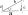
\includegraphics[width=0.25\linewidth]{media/triangle-law-projection.pdf}

\begin{prob}
\item We want to find a pair of orthonormal vectors in the same plane as $\bfa$ and $\bfb$.
  First vector is $\hat{\bfa}$. What is the second vector? (Call it $\hat{\bfc}$
  and find it in terms of $\bfa$ and $\bfb$.)
    
\end{prob}
%\hfill\includegraphics[width=0.25\linewidth]{media/triangle-law-2.pdf}

\newpage
\vspace{10em}
\begin{prob}
  Express the above relationship in terms of matrix vector multiplication so
  that the matrix $M = \begin{bmatrix}
    \bfb^\top \\ \bfa^\top\end{bmatrix}$ can be written in terms of an upper
  triangular matrix and an orthonormal matrix.
\end{prob}

\vspace{10em}

\newpage
\begin{prob}
  Repeat the process for 3 vectors, $\bfa$, $\bfb$ and $\bfc$, and then matrix
  $M = \begin{bmatrix} \bfc^\top \\ \bfb^\top \\ \bfa^\top\end{bmatrix}$. In
  other words, find $\hat{\bfr}_1$, $\hat{\bfr}_2$, $\hat{\bfr}_3$ and write
  them in (upper triangular matrix) (orthonormal matrix) factorization form,
  also known as QR factorization.
\end{prob}
\hfill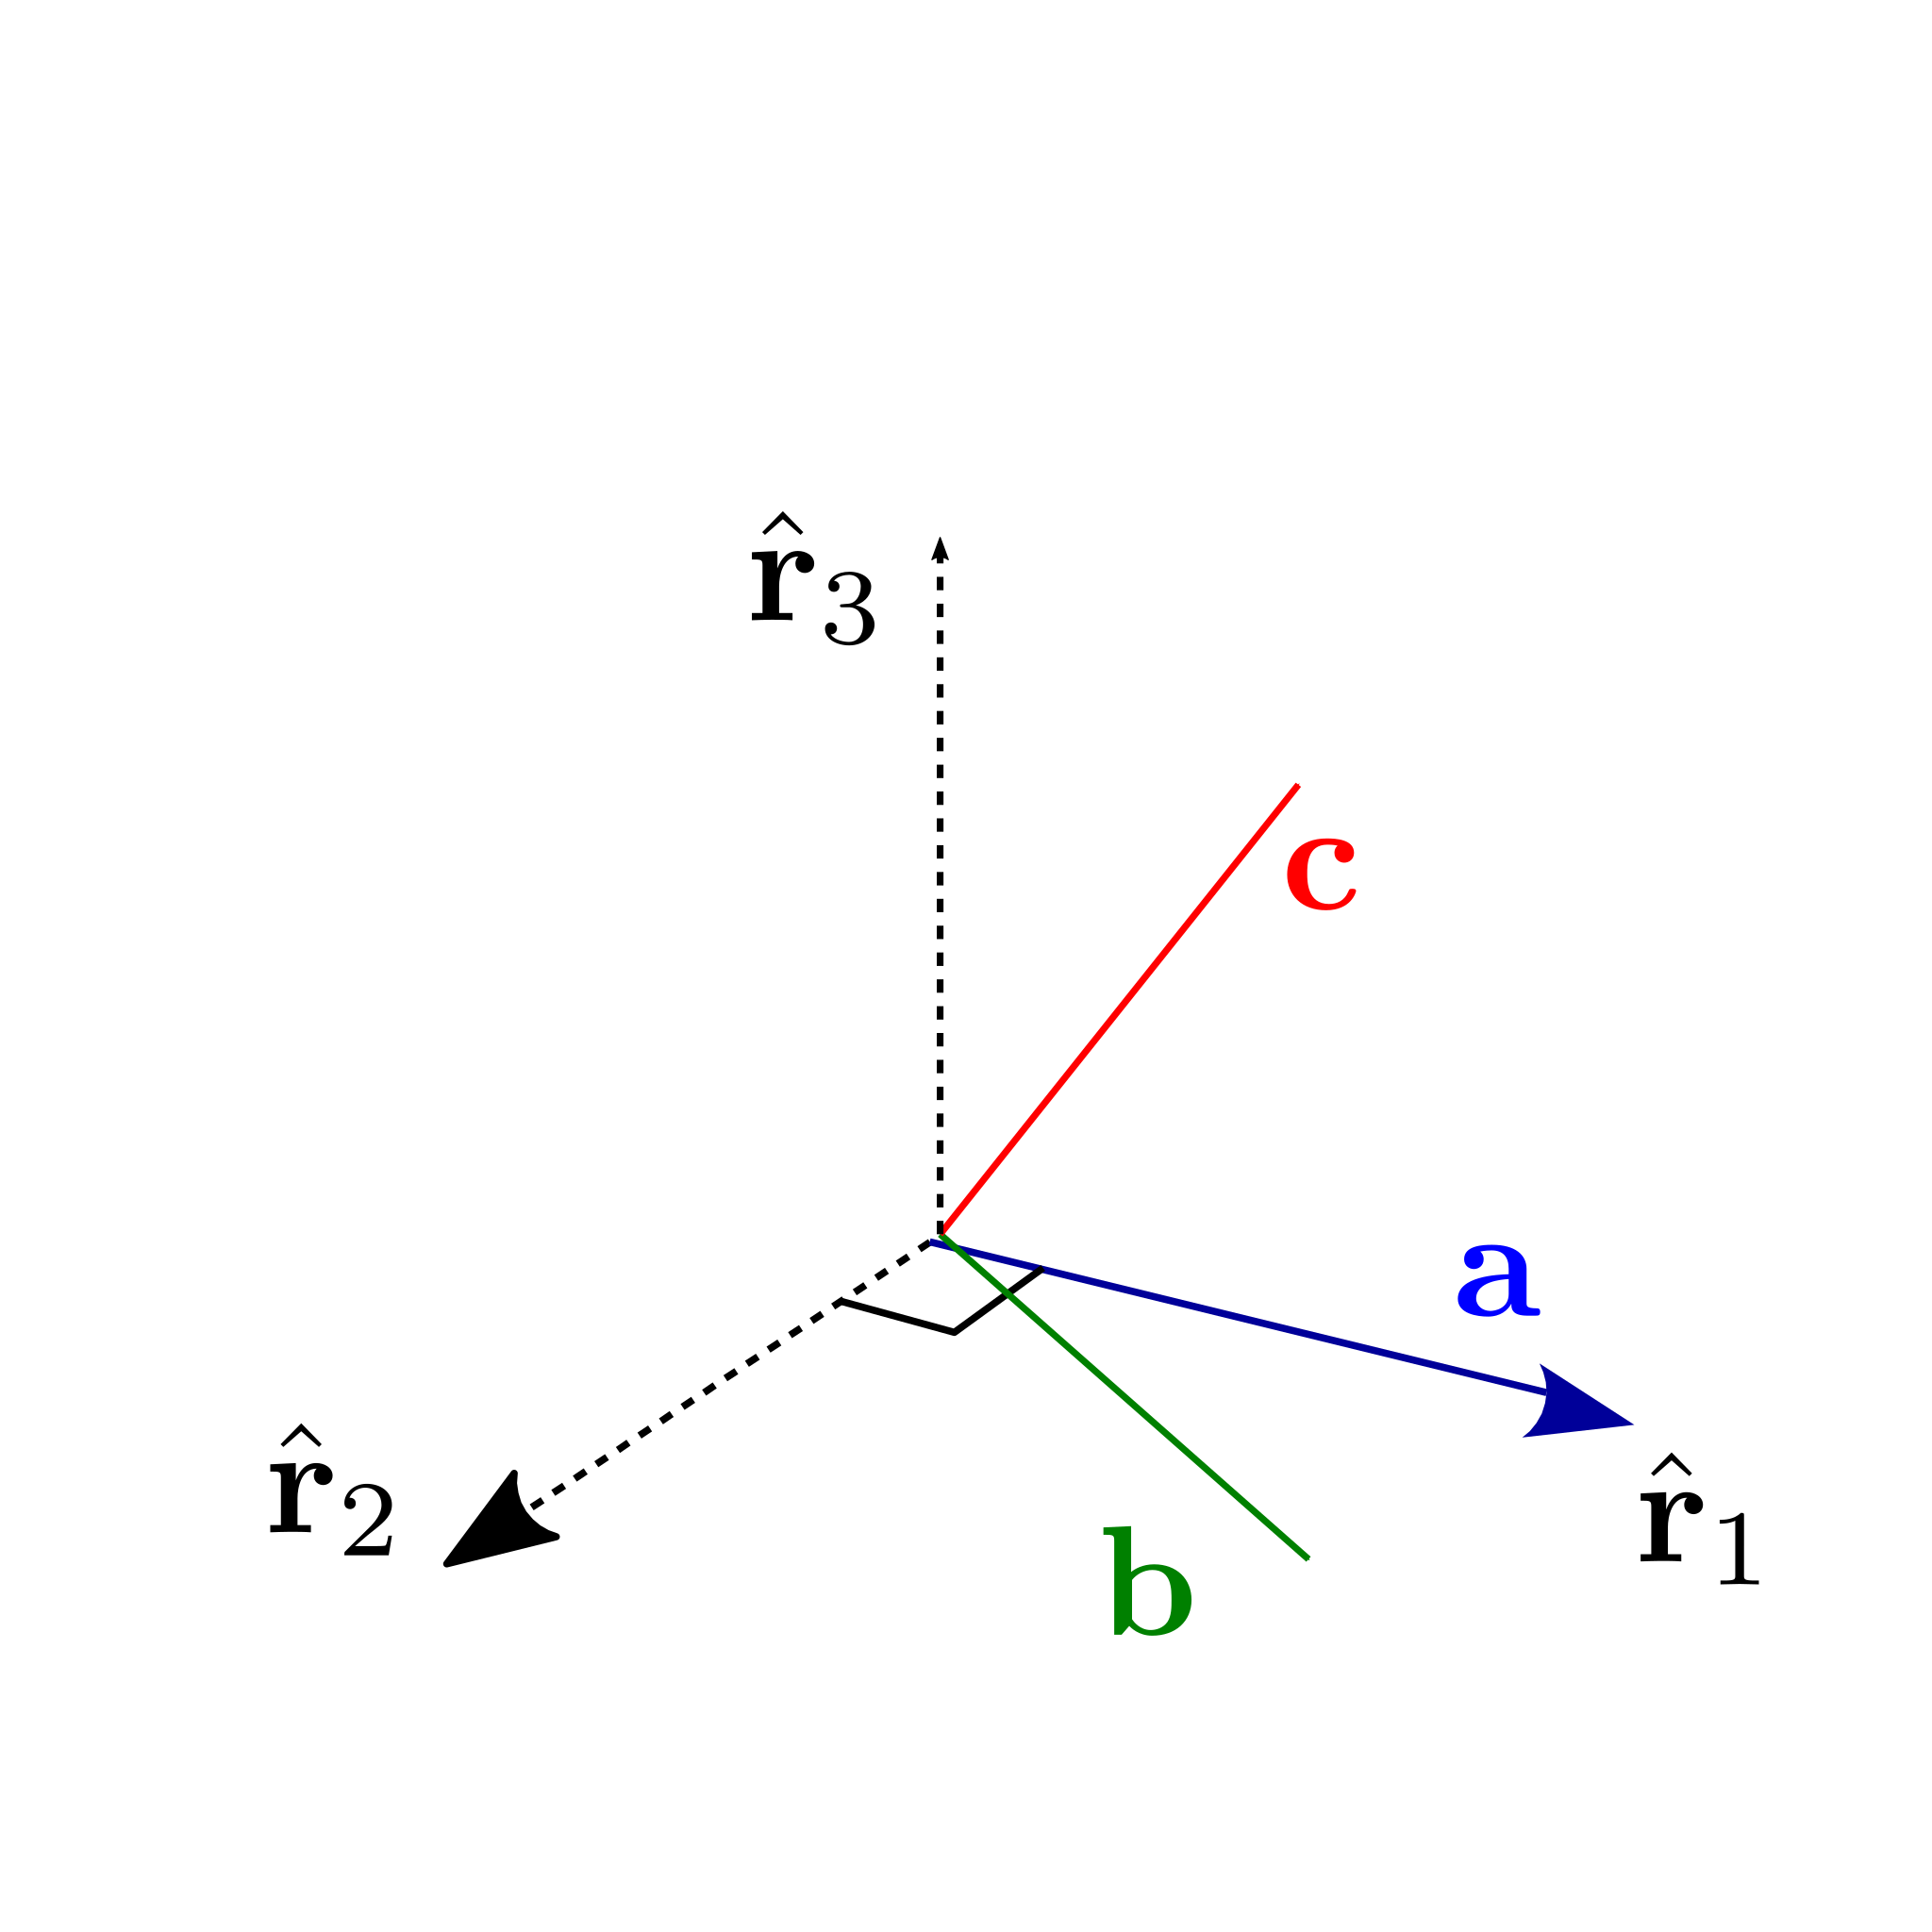
\includegraphics[width=0.5\linewidth]{media/gram-schmidt-3D.pdf}

\begin{enumerate}
  \item Write $\hat{\bfr}_1$ in terms of $\bfa$.
    \vspace{10em}
  \item Write $\hat{\bfr}_2$ in terms of $\bfa$, $\bfb$ and $\hat{\bfr}_1$.
    \vspace{10em}
  \item Write $\hat{\bfr}_3$ in terms of $\bfa$, $\bfb$, $\bfc$, $\hat{\bfr}_1$
    and $\hat{\bfr}_2$.
    \vspace{10em}

\newpage

\item Write the above equations in matrix multiplication form.
  \vspace{10em}
\end{enumerate}

\begin{prob}
  Assuming a QR factorization algorithm is given, find $K, R, \bft$ from $P \in \bbR^{3
    \times 4}$ matrix such that
  \[
  P = \begin{bmatrix}
    KR & K\bft
    \end{bmatrix}
      \]
      and $K \in \bbR^{3 \times 3}$ is an upper triangular matrix, and $R \in
      \bbR^{3 \times 3}$  is a rotation matrix (thus orthonormal) and $\bft \in
      \bbR^{3 \times 1}$ is a translation vector.
  

\end{document}